\section{Logic and Sets}
\subsection{Logic}
\outline

\begin{frame}{Proof by Truth Table}
    \begin{example}
        "$\oplus$" is called \textbf{exclusive or} (xor). $A\oplus B$ is True if and only if $A$ differs from $B$. Prove that $A\oplus B\equiv (\neg A\wedge B)\vee (A\wedge \neg B)$
    \end{example}
    \mypause
    \begin{proof}
        \begin{table}[H]
            \centering
            \begin{tabular}{|c|c|c|c|c|c|}
                $A$ & $B$ & $\neg A\wedge B$ & $A\wedge \neg B$ & $(\neg A\wedge B)\vee (A\wedge \neg B)$ & $A\oplus B$\\\hline\hline
                T & T & F & F & F & F \\
                T & F & F & T & T & T \\
                F & T & T & F & T & T \\
                F & F & F & F & F & F
            \end{tabular}
        \end{table}
    \end{proof}
\end{frame}

\begin{frame}{Reminders for your exam}
    \begin{itemize}
        \item If you want to use truth table, make sure your steps are clear. \textbf{Do not} only list two columns of LHS and RHS. \textbf{Do not} make your truth table look like two copied columns.
        \item Do not use \textbf{01} in truth table; do not use \textbf{Set Notation} in truth table. Make sure the first row consists of propositional logics.
    \end{itemize}
\end{frame}

\begin{frame}{Question 4 in Assignment I}
    \begin{example}
        Suppose that a truth table in n propositional variables is specified. Write the \emph{disjunctive normal form}.
    \end{example}
    \begin{itemize}
        \item In the assignment, as long as you correctly and completely describe the process to get a \emph{disjunctive normal form}, you get full marks.
        \item But it would be better if you could explain why it's a correct transformation.
    \end{itemize}
    \begin{block}{Solution}
        \begin{enumerate}
            \item Pick the rows with true values.
            \item For each row, take the conjunction of true variables and the negation of false variables.
            \item Take the disjunction of these conjunctions.
        \end{enumerate}
    \end{block}
\end{frame}

\begin{frame}{Disjunctive Normal Form}
    \begin{itemize}
        \item First you should know \textbf{why} we need DNF: \textbf{to transform a truth table to a logic expression}. Thus you could use the logic expression for further calculation.
    \end{itemize}
    \begin{example}
        \begin{table}[H]
            \centering
            \begin{tabular}{|c|c|c|}
                $A$ & $B$ & $P(A,B)$\\\hline\hline
                T & T & T \\
                T & F & T \\
                F & T & F \\
                F & F & T
            \end{tabular}
        \end{table}
    \end{example}
    \begin{block}{Solution}
        $$(A\wedge B)\vee(A\wedge\neg B)\vee(\neg A\wedge\neg B)$$
    \end{block}
\end{frame}

\begin{frame}{Some Important Logical Equivalences}
    \begin{block}{Properties}
    \begin{description}[Contraposition]
        \item [Implication] $A\Rightarrow B\equiv \neg A\vee B\equiv \neg B\Rightarrow\neg A$ \textbf{ Important!}
        \item [Distributivity] $A\vee(B\wedge C)\equiv (A\vee B)\wedge(A\vee C)$
        \item [] $A\wedge(B\vee C)\equiv (A\wedge B)\vee(A\wedge C)$
        \item [Absorption] $A\vee (A\wedge B)\equiv A$
        \item [] $A\wedge (A\vee B)\equiv A$
        \item [De Morgan's] $\neg(A\vee B)\Leftrightarrow(\neg A)\wedge(\neg B)$
        \item [] $\neg(A\wedge B)\Leftrightarrow(\neg A)\vee(\neg B)$
        \item [Contraposition] $(A\Rightarrow B)\Leftrightarrow (\neg B\Rightarrow \neg A)$
    \end{description}
    \end{block}
\end{frame}

\begin{frame}{Rules of Inference}
    \begin{itemize}
        \item These rules have fancy latin names, but they are not hard to understand.
        \item You don't need to remember the names of these rules.
    \end{itemize}
     
    \begin{figure}
        \centering
        \begin{subfigure}
            \centering
            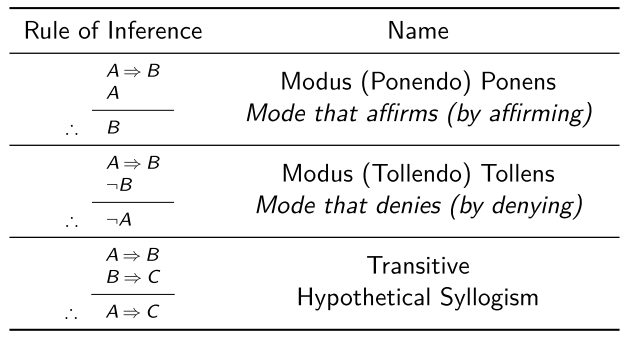
\includegraphics[height=1in]{../images/syllogism1}
        \end{subfigure}%
        ~ 
        \begin{subfigure}
            \centering
            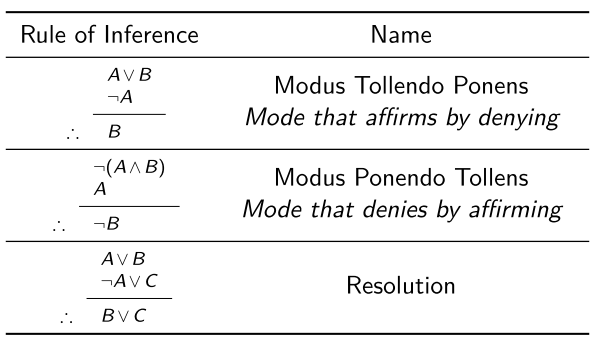
\includegraphics[height=1in]{../images/syllogism2}
        \end{subfigure}
    \end{figure}

    and others...
\end{frame}

\begin{frame}{Arguments in propositional logic}
    \begin{definition}
        An argument is a finite sequence of propositions. All propositions except for the final statement are called \textbf{premises} while the final statement is called the \textbf{conclusion}. We say that an argument is \textbf{valid} if the truth of all premises implies the truth of the conclusion.
    \end{definition}
    
    \begin{columns}[t,onlytextwidth]
        \column{.2\textwidth}
        \begin{center}
            \begin{tabular}{cc}
                &$P_1$\\
                &$\vdots$\\
                &$P_n$\\\hline
                $\therefore$ & $C$
            \end{tabular}
        \end{center}

        \column{.8\textwidth}
        \begin{itemize}
            \item 
            i.e. $(P_1\wedge P_2\cdots\wedge P_n)\Rightarrow C$ is a tautology. Note that it \textbf{does not} mean that $C$ is always true!
            \item
            To disprove the validness, make all of the premises true but the conclusion wrong.
            \item
            To disprove the validness, providing a counterexample is a wiser strategy than long proofs.
        \end{itemize}
        \end{columns}
\end{frame}

\begin{frame}{Arguments in propositional logic}
    \begin{definition}
        If, in addition to being valid, an argument has only true premises, we say that the argument is \textbf{sound}. In that case, its conclusion is \textbf{true}.
    \end{definition}
    \mypause
    \begin{itemize}
        \item Hence, to disprove the soundness, you only need to find \textbf{a false premise}.
        \item To make a valid argument sound, make all the premises true by \textbf{assigning the variables} properly.
    \end{itemize}
\end{frame}

\begin{frame}{Predicate Logic}
    \begin{itemize}
        \item When using quantifiers $\forall$ and $\exists$, pay attention to the order.
        \item $\forall x\exists y P(x,y)$ is different from $\exists y\forall x P(x,y)$
        \item $\forall xP(x)\vee \forall xQ(x)$ is different from $\forall x(P(x)\vee Q(x))$
        \item If you are creating a counterexample, do not involve other variables than $A$ in $P(A)$. For example, do not define $P(x)$ as $x>1$ and $y<1$.
        \item You cannot change the \textbf{domain of disclosure} after you define it.
    \end{itemize}
    \textbf{Some mistakes:}
    \begin{example}
        Let the domain of $Q(x)$ be $x\in\mathbb{N}$. $Q(x)$ is true if $x\geq 0$. Thus $\exists x Q(x)$ is true (so far everything is fine).
        
        $\cdots$ Then on the right hand side, let $w<0$. Thus $\exists w Q(w)$ is false (\textbf{no!}).
    \end{example}
\end{frame}

\begin{frame}{Vacous Truth}
    \begin{block}{Vacuous Truth}
        If the domain of the universal quantifier $\forall$ is the empty set $M=\emptyset$, then the statement $(\forall x\in M)A(x)$ is defined to be true.
    \end{block}
    \begin{itemize}
        \item Remind the definition of \textbf{Chain Complete}. Why a chain complete poset has the least element?
        \item Empty chain, due to vacuous truth, is also a chain.
    \end{itemize}
\end{frame}

\begin{frame}{Tips for your exam}
    \begin{itemize}
        \item If you replace symbols like $\Leftrightarrow$ and $\Rightarrow$ with $\vee$, $\wedge$ or $\neg$, the expression might be terribly longer.
        \item So before you do terrible calculations, try proving by rules of inference. "Maybe" you can avoid tedious calculations.
    \end{itemize}
\end{frame}

\subsection{Set Theory}
\outline

\begin{frame}{Subsets}
    \begin{itemize}
        \item  $X = Y$ if and only if $X \subseteq Y$ and $Y \subseteq X$.
    \end{itemize}
    \begin{definition}
        We say that $X$ is a proper subset of $Y$ if $X \subseteq Y$ but $X \neq Y$. In that case we write $X \subset Y$.
    \end{definition}
    \begin{itemize}
        \item Pease use $\subset$ to denote proper subset in your assignments and exams rather than $\subsetneq$.
    \end{itemize}
\end{frame}

\begin{frame}{Powerset and Cardinality}
    \begin{definition}
        If a set has a finite number of elements, we define the \textbf{cardinality} of $X$ to be this number, denoted by $|X|$.
    \end{definition}
    \begin{definition}
        If X is a set, then the \textbf{power set} of X, denoted $\mathscr{P}(X)$, is the set of all subsets of X. I.e. $$\mathscr{P}(X) = \{A | A \subseteq X\}$$
        This means the expressions $A \in \mathscr{P}(X)$ and $A \subseteq X$ are equivalent.
    \end{definition}
\end{frame}

\begin{frame}{Operations on Sets}
    \begin{itemize}
        \item Proof by Venn Diagram will earn 0 point.
        \item If you want to use $\overline{A}$ to denote $A^c$, define this notation and denote the $M$ at first.
        \item Do not misuse $\wedge$ and $\cap$; $\vee$ and $\cup$.
        \item Before you replace $\backslash$ with $\wedge$ and $^c$, try using the properties below. Make your calculations as simple as possible.
    \end{itemize}
    \begin{block}{Properties}
    \begin{itemize}
        \item $(A\cup B)\m C=(A\m C)\cup(B\m C)$
        \item $(A\cap B)\m C=(A\m C)\cap(B\m C)$
        \item $A\m (B\cup C)=(A\m B)\cap(A\m C)$
        \item $A\m (B\cap C)=(A\m B)\cup(A\m C)$
        \item $A\m B=B^c\cap A$
        \item $(A\m B)^c=A^c\cup B$
    \end{itemize}
    \end{block}
\end{frame}

\begin{frame}{Cartesian Product of Sets}
    \begin{definition}
        $$A\times B:=\{(a,b)|a\in A\wedge b\in B\}$$
        $A\times B$ is called the cartesian product of $A$ and $B$.
    \end{definition}
    \begin{itemize}
        \item It's easy to define ordered n-tuples $A_1\times A_2\times\cdots\times A_n$
        \item $A^n$ is short for $A\times\cdots\times A$
        \item The cartesian product of some sets is still a set
    \end{itemize}
\end{frame}

\begin{frame}{Cartesian Product of Sets}
    \textbf{Some mistakes:}
    \begin{example}
        Any subset of $\mathbb{N}\times \mathbb{N}$ can be written as $A\times B$ (\textbf{no!})
    \end{example}
\end{frame}

\begin{frame}{Russell's Paradox}
    \begin{theorem}
        The set of all sets that are not members of themselves is not a set. I.e. $$R:=\{x|x\notin x\} \text{ is not a set}$$
    \end{theorem}
    \begin{proof}
        If $R\in R$, then $R$ should satisfy $R\notin R$ by definition. 
        
        If $R\notin R$, then it should be put in $R$ by definition.

        Both of the assumptions lead to contradiction.
    \end{proof}
    \begin{itemize}
        \item Similar proof is useful in other questions (in \emph{Cantor's Theorem})
        \item To prove something related to sets, you may \textbf{construct a "set"} with particular constraints, and \textbf{substitute this "set" back} to our hypothesis. Finally it leads to contradiction.
    \end{itemize}
\end{frame}

\begin{frame}{Keep Calm and Carry on!}
    \begin{figure}
        \centering
        
\includegraphics[width=1.4in]{../images/duckling}
        \caption{Zach's little reward for Mid 1 High!}
    \end{figure}
\end{frame}